\chapter{Descrição do sistema de controle}

O presente trabalho busca controlar a posição de um carro ao longo de uma guia linear. Para realizar essa tarefa, foi escolhida a realimentação de estados como estratégia de controle. Essa forma de controle é descrita na sequência.

\section{Realimentação de Estados}

Na realimentação de estados a entrada da planta é calculada da seguinte forma: são determinados requisitos para o sistema, de tal forma que esses correspondem a novos polos do sistema no plano complexo; para tal, uma lei de controle para a mudança dos polos é estabelecida, em que  

\begin{equation}
    U(k) = -K (X(k) - X_{ss}) + U_{ss}
    \label{vetor_controle_realimentacao}
\end{equation}

\noindent em que $K$ é o vetor de controle, $K \in \mathbb{R}^{n_u n_x}$, sendo

\begin{equation}
    X_{ss} = N_x r_{rss}
\end{equation}

\begin{equation}
    U_{ss} = N_u r_{rss}
\end{equation}

\noindent em que $r_{ss}$ é uma referência constante para a saída, $N_x$ e $N_u$ são elementos ajutados para garantir que, em regime estacionário, a saída seja igual a referência. Mais ainda, $k$ é o índice de tempo discreto. 

A Figura \ref{fig:diagrama_blocos} apresenta o diagrama de blocos com a presença do controlador via realimentação de estados.

\begin{figure}[H]
    \centering
    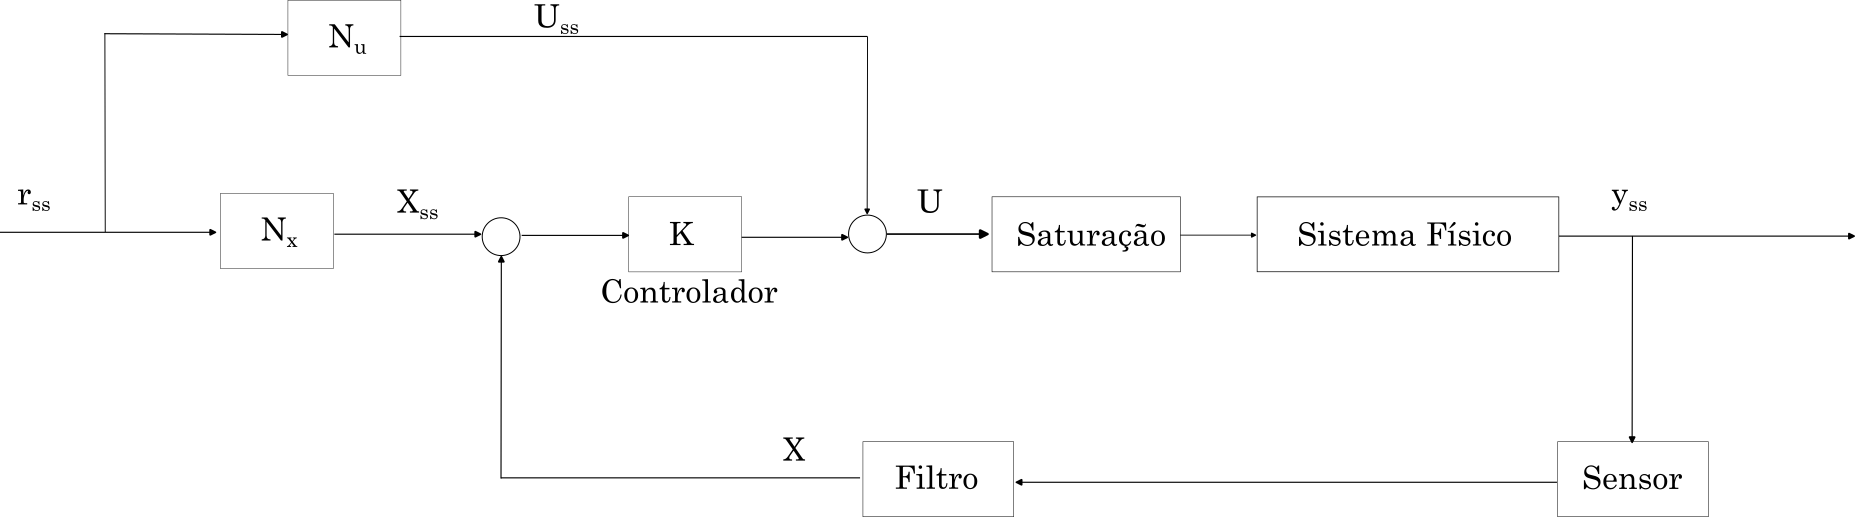
\includegraphics[width=1\linewidth]{figuras/diagrama_blocos.png}
    \caption[Diagrama de blocos da planta]{Diagrama de blocos da planta.}
    \label{fig:diagrama_blocos}
\end{figure}

Conforme mostrado na Figura \ref{fig:diagrama_blocos}, a variável de controle (\textit{U}) está sujeita a saturação. No caso do sistema estabelecido, a variável de controle é a tensão aplicada no motor CC, medida em Volts, podendo operar na faixa de -12 V a +12 V.

Como a lei de controle (\ref{vetor_controle_realimentacao}) é baseada em tempo discreto, deve-se obter uma representação do sistema no espaço de estados a tempo discreto. Isso é realizado na sequência.

\section{Representação no Espaço de Estados a tempo discreto}

No capítulo anterior foi elaborado e validado o modelo do espaço de estados a tempo contínuo, unindo as Equações (\ref{espaco_estados}) e (\ref{espaco_estados_saida}) com os valores obtidos, obtém-se o seguinte modelo:

\begin{gather}
    \begin{bmatrix}
        \dot{x}_c(t) \\ \ddot{x}_c(t)
    \end{bmatrix}=
    \begin{bmatrix}
        0 && 1 \\ 0 && -5,93
    \end{bmatrix}
    +
    \begin{bmatrix}
        x_c(t) \\ \dot{x}_c(t)
    \end{bmatrix}
    \begin{bmatrix}
        0 \\ 0,90
    \end{bmatrix}
    Vm(t)
    \label{espaco_estados1}
\end{gather}

\begin{gather}
    Y(t)=
    \begin{bmatrix}
        1 && 0
    \end{bmatrix}
    \begin{bmatrix}
        x_c(t) \\ \dot{x}_c(t)
    \end{bmatrix}
    \label{espaco_estados_saida1}
\end{gather}

Com o modelo em mãos, se torna necessário discretizar a planta para elaboração e implementação do controlador. A tempo discreto, pode-se representar o sistema do seguinte modo:

\begin{equation}
    P :\begin{cases} 
        X(k+1) = \Phi X(k) + \varGamma U(k) \\
        Y(k) = CX(k) + DU(k) \\
        \end{cases}
    \label{modelo_espaco_estados_discreto}
\end{equation}

\noindent em que $\Phi$, $\Gamma$ são matrizes do sistema a tempo discreto, considerando um período de amostragem $T_s$.

Buscando um bom desempenho do controlador ao mesmo tempo com um custo de implementação baixo, foi decidido que o período de amostragem seria

\begin{equation}
    T_s = 10 \textnormal{ ms}
    \label{periodo_amostragem}
\end{equation}

As Equações (\ref{espaco_estados1}) e (\ref{espaco_estados_saida1}) foram discretizadas utilizando o método segurador de ordem zero \cite{franklin2013sistemas}. Assim, a tempo discreto, o sistema é representado por

\begin{gather}
    X(k+1)=
    \begin{bmatrix}
        1 && 0,0097 \\ 0 && 0,9424
    \end{bmatrix}
    X(k)
    +
    \begin{bmatrix}
        0 \\ 0,0087
    \end{bmatrix}
    U(k)
    \label{espaco_estados_d}
\end{gather}

\begin{gather}
    Y(k)=
    \begin{bmatrix}
        1 && 0
    \end{bmatrix}
    X(k)
    \label{espaco_estados_saida_d}
\end{gather}

\section{Projeto da realimentação de estados}

Considerando um sistema de segunda ordem no caso submortecido, adotar-se-ão os seguintes requisitos de desempenho: tempo de pico $t_p$ e máximo sobressinal $M_s$. Sabe-se que a relação entre $t_p$, $M_s$, o fator de amortecimento $\zeta$ e a frequência natural $w_n$ do sistema são dados por \cite{ogata2010engenharia}

\begin{equation}
    t_p=\frac{\pi}{w_n \sqrt{1-\zeta^2}}
    \label{tempo_pico}
\end{equation}

\begin{equation}
    M_s=e^\frac{-\zeta \pi}{\sqrt{1-\zeta^2}}
    \label{maximo_sobressinal}
\end{equation}

Foram estipulados como requisitos para o sistema um máximo sobressinal de 80\% e 0,3 segundos como tempo de pico ($t_p=0,3$). Com esses valores, as Equações (\ref{tempo_pico}) e (\ref{maximo_sobressinal}) formam um sistema de equações com 2 variáveis, isolando $\zeta$ e $w_n$ obtêm-se

\begin{equation}
    \zeta = \sqrt{\frac{\ln(M_s)^2}{\pi^2+\ln(M_s)^2}} =  0,06
    \label{zeta}
\end{equation}

\begin{equation}
    w_n = \frac{\pi}{t_p \sqrt{1-\zeta^2}} = 9,83
    \label{wn}
\end{equation}

Agora com os valores de $w_n$ e $\zeta$, os polos de malha fechada associados o desempenho desejado são

\begin{equation}
    s_{polos} = -\zeta w_n \pm w_n \sqrt{1-\zeta^2}
    \label{polos_malha_fechada}
\end{equation}

\noindent resultando nos seguintes polos a tempo contínuo:

\begin{equation}
    s_{polos} = -0,58 \pm 9,82 j
    \label{polos_continuo}
\end{equation}

Esses polos são convertidos para o tempo discreto por meio da seguinte equação:

\begin{equation}
    z_{polos} = e^{(s T_s)} = 0,9894 \pm 0,0974 j
    \label{polos_discreto}
\end{equation}

A partir de (\ref{polos_continuo}), pode-se escrever a equação característica desejada para o sistema

\begin{equation}
    z^2-1,9788z+0,0095 = 0
    \label{equacao_desejada}
\end{equation}

Agora com os polos obtidos para o desempenho desejado, torna-se possível realizar o projeto da realimentacão de estados. Substituindo a Equação (\ref{vetor_controle_realimentacao}) em (\ref{modelo_espaco_estados_discreto}), tem-se

\begin{equation}
     X(k+1) = \Phi X(k) - \varGamma KX(k) = (\Phi-\varGamma K)X(k)
     \label{modelo_espaco_estados_discreto2}
\end{equation}

\noindent em que os polos de malha fechada são determinados resolvendo-se:

\begin{equation}
    | z I_2 - (\Phi-\varGamma K) | = 0
    \label{polos_MF}
\end{equation}

Igualando as Equações (\ref{polos_MF}) e (\ref{equacao_desejada}) pode-se obter os valores do controlador para realimentacão de estados.

\begin{equation}
    | z I_2 - (\Phi-\varGamma K) | = z^2-1,9788z+0,0095
    \label{realimentacao_estados}
\end{equation}

Dessa forma, determinou-se o seguinte vetor de realimentação de estados:

\begin{equation}
    K = 
    \begin{bmatrix}
        110,3976 && -4,7399
    \end{bmatrix}
    \label{controlador_realimentacao}
\end{equation}

O cálculo de $N_x$ e $N_u$ é realizado de modo a garantir que $y_{ss} = r_{ss}$, sendo que  $y_{ss}$ e $r_{ss}$ representam a saída da planta e a referência em regime estacionário. Especificamente, esses elementos são determinados como se segue \cite{franklin2013sistemas}:

\begin{equation}
    \begin{bmatrix}
        N_x \\ N_u
    \end{bmatrix}
    =
    \begin{bmatrix}
        \phi-I_2 && \varGamma \\ C && 0
    \end{bmatrix}
    ^{-1}
    \begin{bmatrix}
        0 && 0 && 1
    \end{bmatrix}
    =
    \begin{bmatrix}
        1 \\ 0 \\ 0
    \end{bmatrix}
    \label{ganhos_Nxu}
\end{equation}

\noindent assim, 

\begin{equation}
    N_x = 
    \begin{bmatrix} 
        1 \\ 0 
    \end{bmatrix}
    \label{Nx}
\end{equation}

\begin{equation}
    N_u = 
    \begin{bmatrix} 
        0 
    \end{bmatrix}
    \label{Nu}
\end{equation}

Dessa forma, considerando que tanto a posição quanto a velocidade do carro são medidas, a entrada da planta é calculada em malha fechada da seguinte forma:

\begin{equation}
    U(k) = 
    \begin{bmatrix}
        110,3976 && -4,7399
    \end{bmatrix}
    \left(X(k) - 
    \begin{bmatrix}
        1 \\ 0 
    \end{bmatrix}
    r_{ss} \right)
    \label{vetor_controle_realimentacao_calculado}
\end{equation}